\section{Finding Limits and Characterizing Delay}
\label{sec:delay_char}
As explained in Section \ref{sec:qoi_model}, delay of a flow can be expressed as
\begin{equation}
	D = \frac{ k_{req} \cdot I_S \cdot CF \cdot TF}{W} + \frac{P_S \cdot DF \cdot (PL-1)}{W}
\end{equation}
%We will make some substitutions to get the following version
%\begin{equation}
%	D = \frac{ P_S \cdot CF \cdot P_N \cdot TF}{W} + \frac{P_S \cdot DF \cdot (PL-1)}{W}
%\end{equation}
%
Let $PL()$ be a function that provides the path length between $i$ and $j$, and let $TF_{i}^{j}$ be a random variable of the Traffic Factor for the bottleneck node between $i$ and $j$, i.e. the node along the path from $i$ to $j$ with the highest $u_x$.  Finally, let $P_N$ be a random variable that describes the number of packets in a given request, capturing both the possible randomness of $k_{req}$ and $I_S$.  
Then, building on the equation for delay above and making some substitutions, we can get the following equation to describe the delay from a node $i$ given a destination of $j$:
\begin{equation}
	D_{i}^{j} = \frac{ P_S \cdot CF \cdot P_N \cdot TF_{i}^{j}}{W}  + \frac{P_S \cdot DF \cdot (PL(i,j)-1)}{W}
\end{equation}

%Also, recall that $TF$ is a random variable of the flows being forwarded at the bottleneck node along the path of the flow.  
Defining two constants to simplify the expression,
\begin{eqnarray*}
	C_1 = \frac{P_S \cdot CF}{W} \\
	C_2 = \frac{P_S \cdot DF}{W}
\end{eqnarray*}
we can express the delay as
\begin{equation}
	D_{i}^{j} = C_1 \cdot P_N \cdot TF_{i}^{j} + C_2 \cdot PL(i,j)
\end{equation}

We can develop an expression for a distribution of delay as follows.  First, we define the cumulative distribution of a source-destination pair $(i,j)$:
\begin{equation*}
	P( D_{i}^{j} \leq d ) = P( C_1 \cdot P_N \cdot TF_{i}^{j} + C_2 \cdot PL(i,j) \leq d )
\end{equation*}
\begin{equation*}
	= P( P_N \cdot TF_{i}^{j} \leq \frac{d - C_2 \cdot PL(i,j)}{C_1}  )
\end{equation*}
Next, conditioning over all possible values of $TF$, we get
\begin{eqnarray*}
	&&P( D_{i}^{j} \leq d ) = \\
	&&\sum\limits_{\tau = 1}^{\tau_{max}} P( P_N \cdot TF \leq \frac{d - C_2 \cdot PL(i,j)}{C_1} | TF = \tau ) \cdot f_{TF_{i}^{j}}(\tau)
\end{eqnarray*}
%\begin{equation*}
%	P( D_{i}^{j} \leq d ) = \sum\limits_{\tau = 1}^{\tau_{max}} P( P_N \cdot TF \leq \frac{d - C_2 \cdot PL(i,j)}{C_1} | TF = \tau ) \cdot f_{TF_{i}^{j}}(\tau)
%\end{equation*}
\begin{equation*}
	= \sum\limits_{\tau = 1}^{\tau_{max}} P( P_N \leq \frac{d - C_2 \cdot PL(i,j)}{C_1 \cdot \tau} ) \cdot f_{TF_{i}^{j}}(\tau)
\end{equation*}
Substituting the cumulative distribution representing the data load, $F_{P_{N}}$:
\begin{equation*}
	F_{D_{i}^{j}}(d) = \sum\limits_{\tau = 1}^{\tau_{max}} F_{P_N}( \frac{d - C_2 \cdot PL(i,j)}{C_1 \cdot \tau} ) \cdot f_{TF_{i}^{j}}(\tau)
\end{equation*}
Then, we can generalize the expression to give a distribution for a flow originating in node $i$ with an unknown destination by conditioning over all possible destinations, $j$.
\begin{equation}
\label{eq:delay_dist_pdf_i}
	F_{D_i} = \sum\limits_{j \neq i} [ \sum\limits_{\tau = 1}^{\tau_{max}} F_{P_N}( \frac{d - C_2 \cdot PL(i,j)}{C_1 \cdot \tau} ) \cdot f_{TF_{i}^{j}}(\tau) ] \cdot p(j)
\end{equation}
Finally, we can get an average distribution of all flows' delays by summing over all sources and dividing by the the number of sources.  This average delay distribution is in Equation (\ref{eq:full_delay_cdf}).

\begin{figure*}[!t]
%\setcounter{equation}{9}
\begin{equation}
\label{eq:full_delay_cdf}
	F_D(d) = \frac{1}{N} \cdot \sum\limits_{i = 1}^N \sum\limits_{j \neq i} \sum\limits_{tf=1}^{tf_{max}}  F_{P_N}( \frac{d - C_2 \cdot PL(i,j)}{C_1 \cdot p_N} ) \cdot f_{TF_{i | j}}( tf ) \cdot p(j)
\end{equation}
\end{figure*}
%\setcounter{equation}{5}

%\begin{figure*}[!t]
%\begin{equation}
%\label{eq:full_delay_cdf}
%	F_D(d) = \frac{1}{N} \cdot \sum\limits_{i = 1}^N \sum\limits_{j \neq i} \sum\limits_{tf=1}^{tf_{max}}  F_{P_N}( \frac{d - C_2 \cdot PL(i,j)}{C_1 \cdot p_N} ) \cdot f_{TF_{i | j}}( tf ) \cdot p(j)
%\end{equation}
%\end{figure*}

\begin{figure}[]
\centering
       \subfigure[Line Network, $N = 40$, $I_S = 36 KB$]{
%        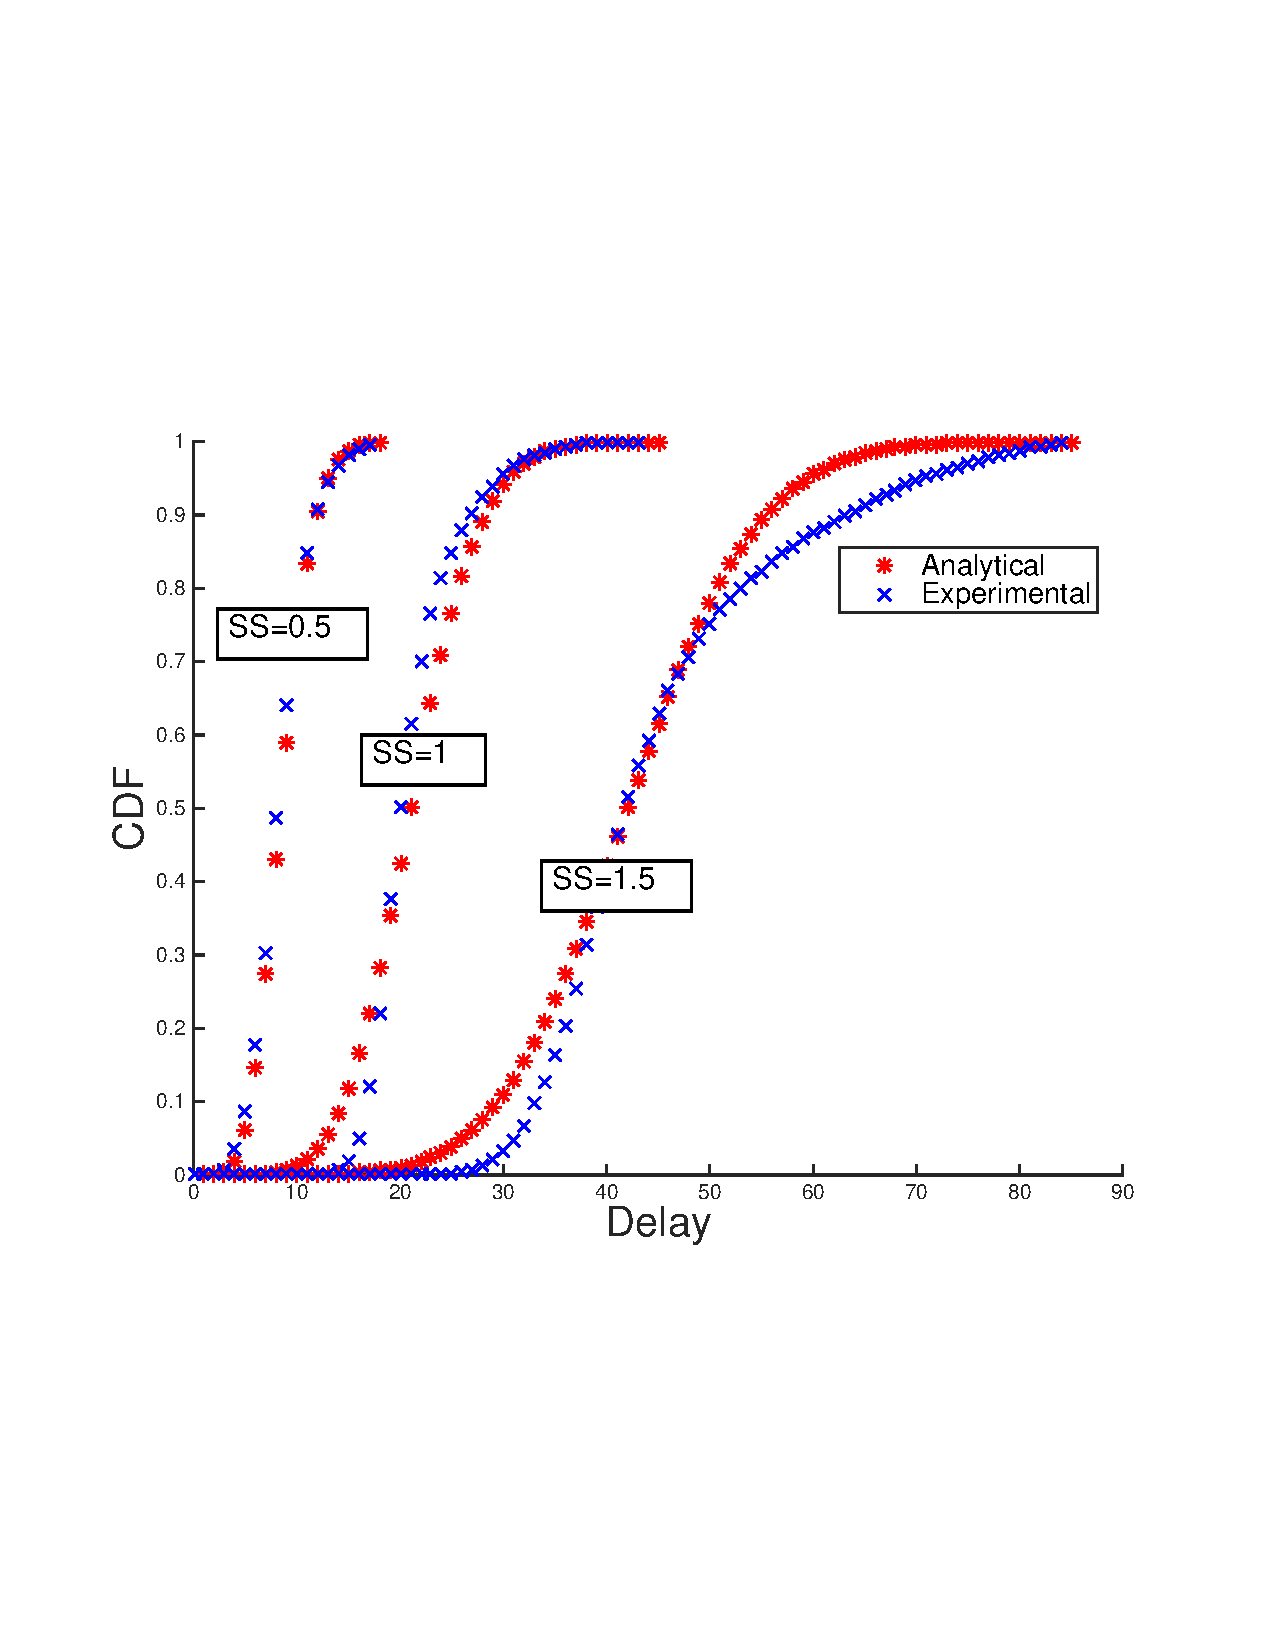
\includegraphics[scale=0.40, clip=true, trim=12mm 65mm 20mm 65mm]{figures/delay_cdfs/delay_cdf_line.pdf}
%        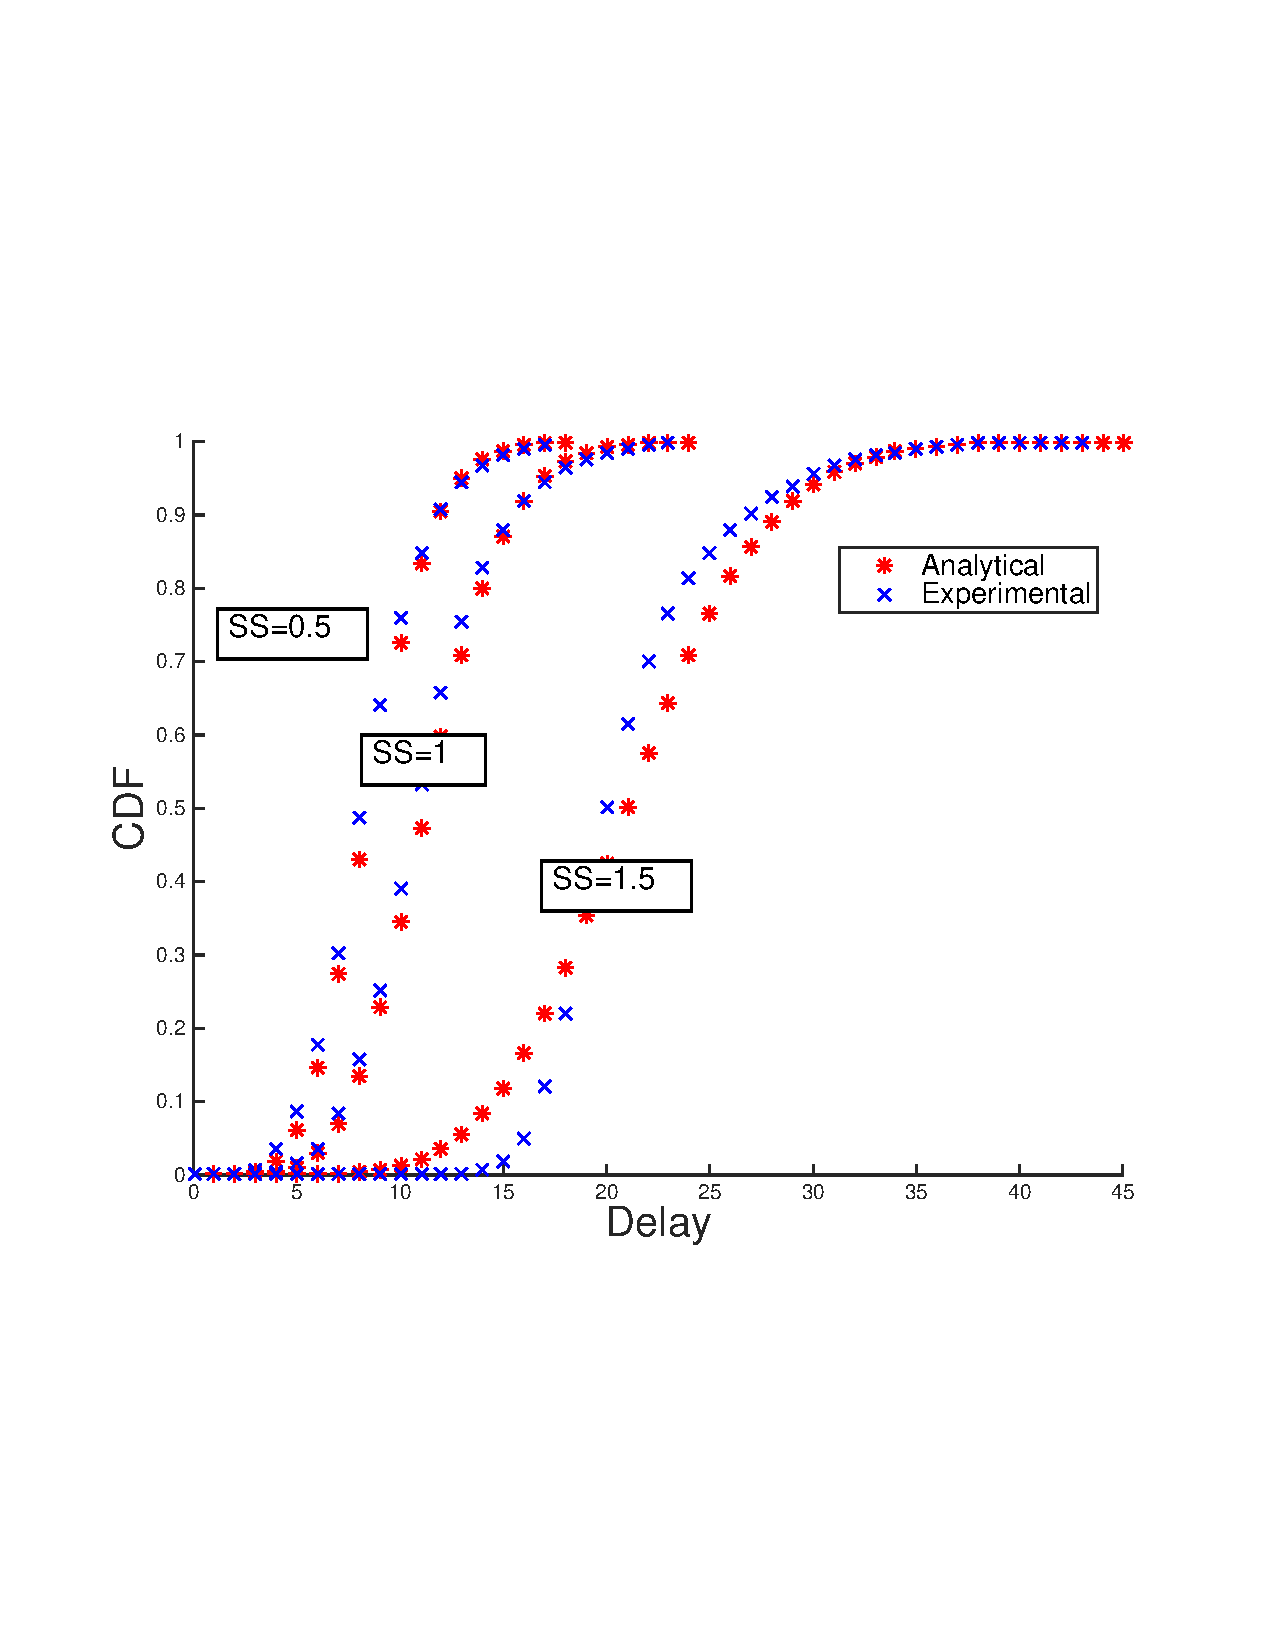
\includegraphics[scale=0.40, clip=true, trim=12mm 65mm 20mm 65mm]{figures/delay_cdfs/delay_cdf_line_full_2.pdf}
        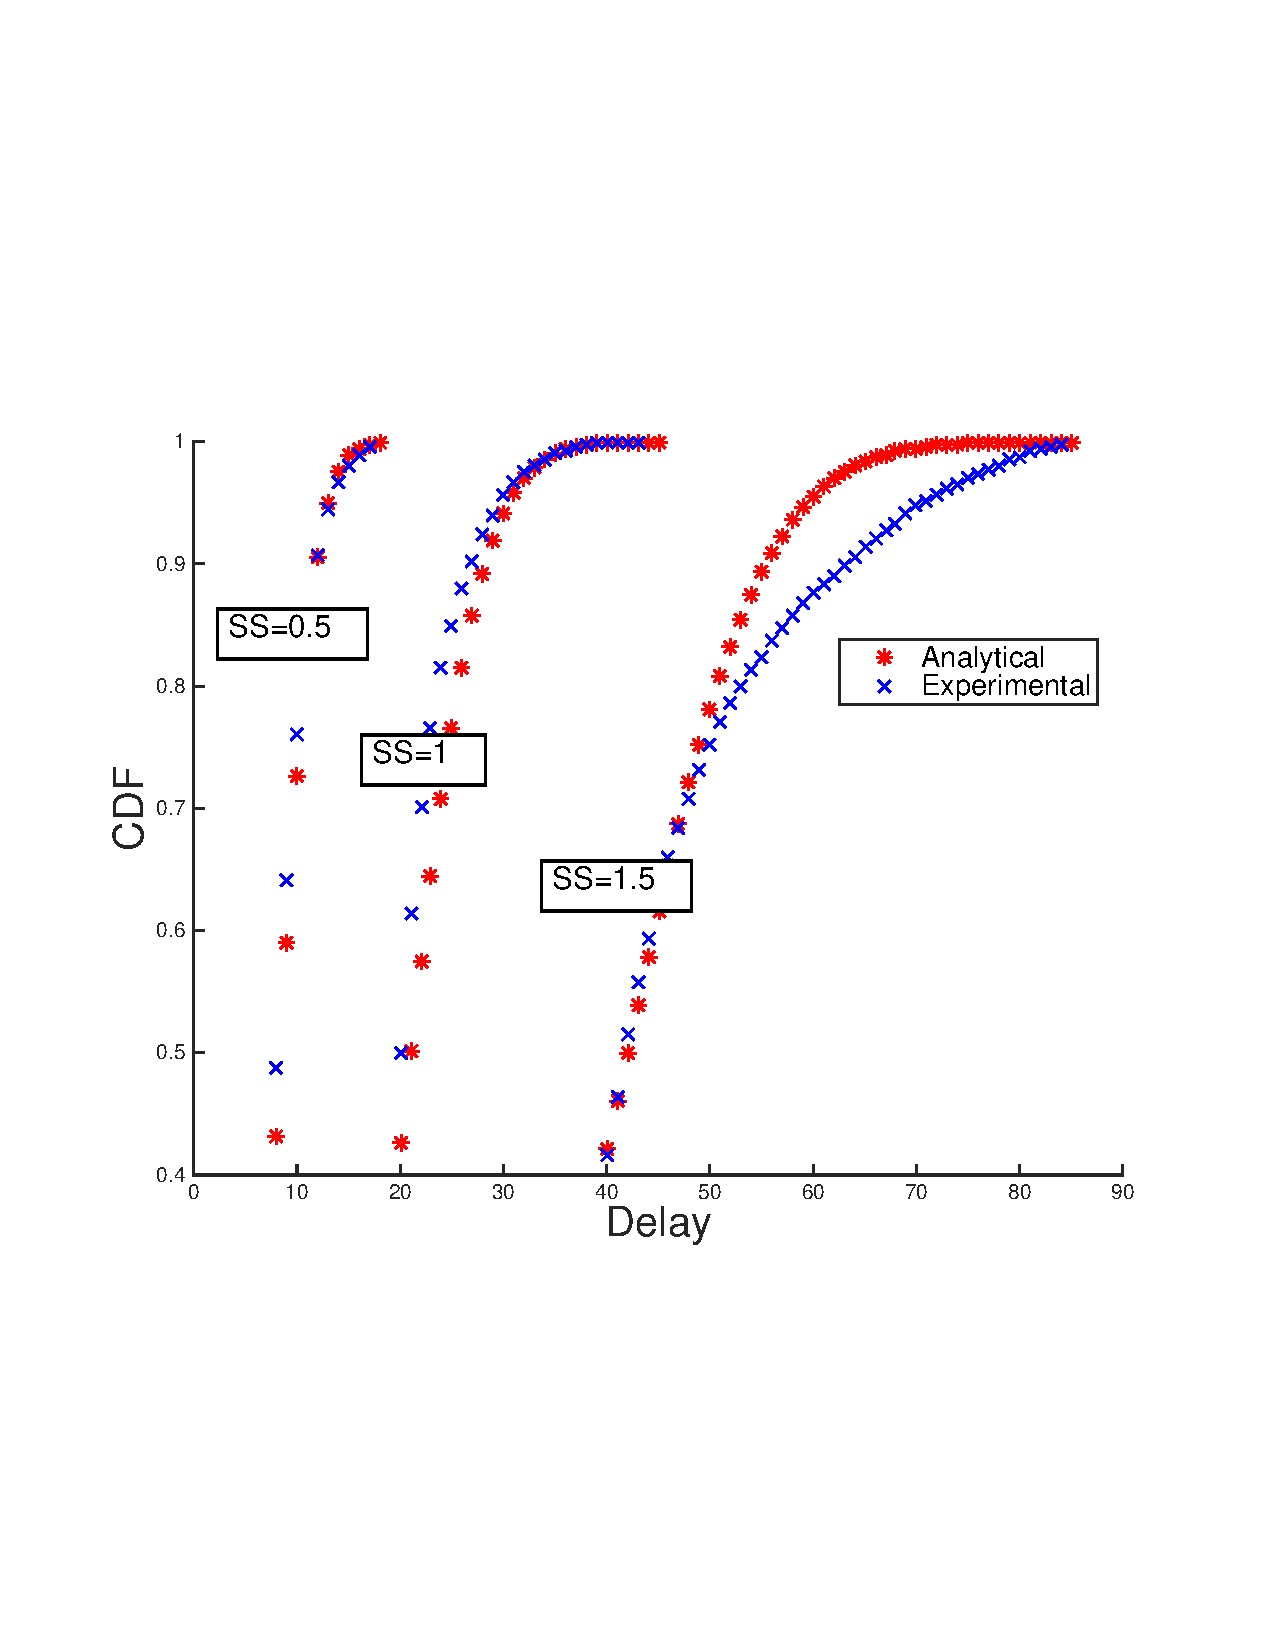
\includegraphics[scale=0.40, clip=true, trim=12mm 65mm 20mm 65mm]{figures/delay_cdfs/delay_cdf_line_half.pdf}
        \label{fig:delay_cdf_line}
        }
    \subfigure[Grid Network, $N = 49$, $I_S = 72 KB$]{
%        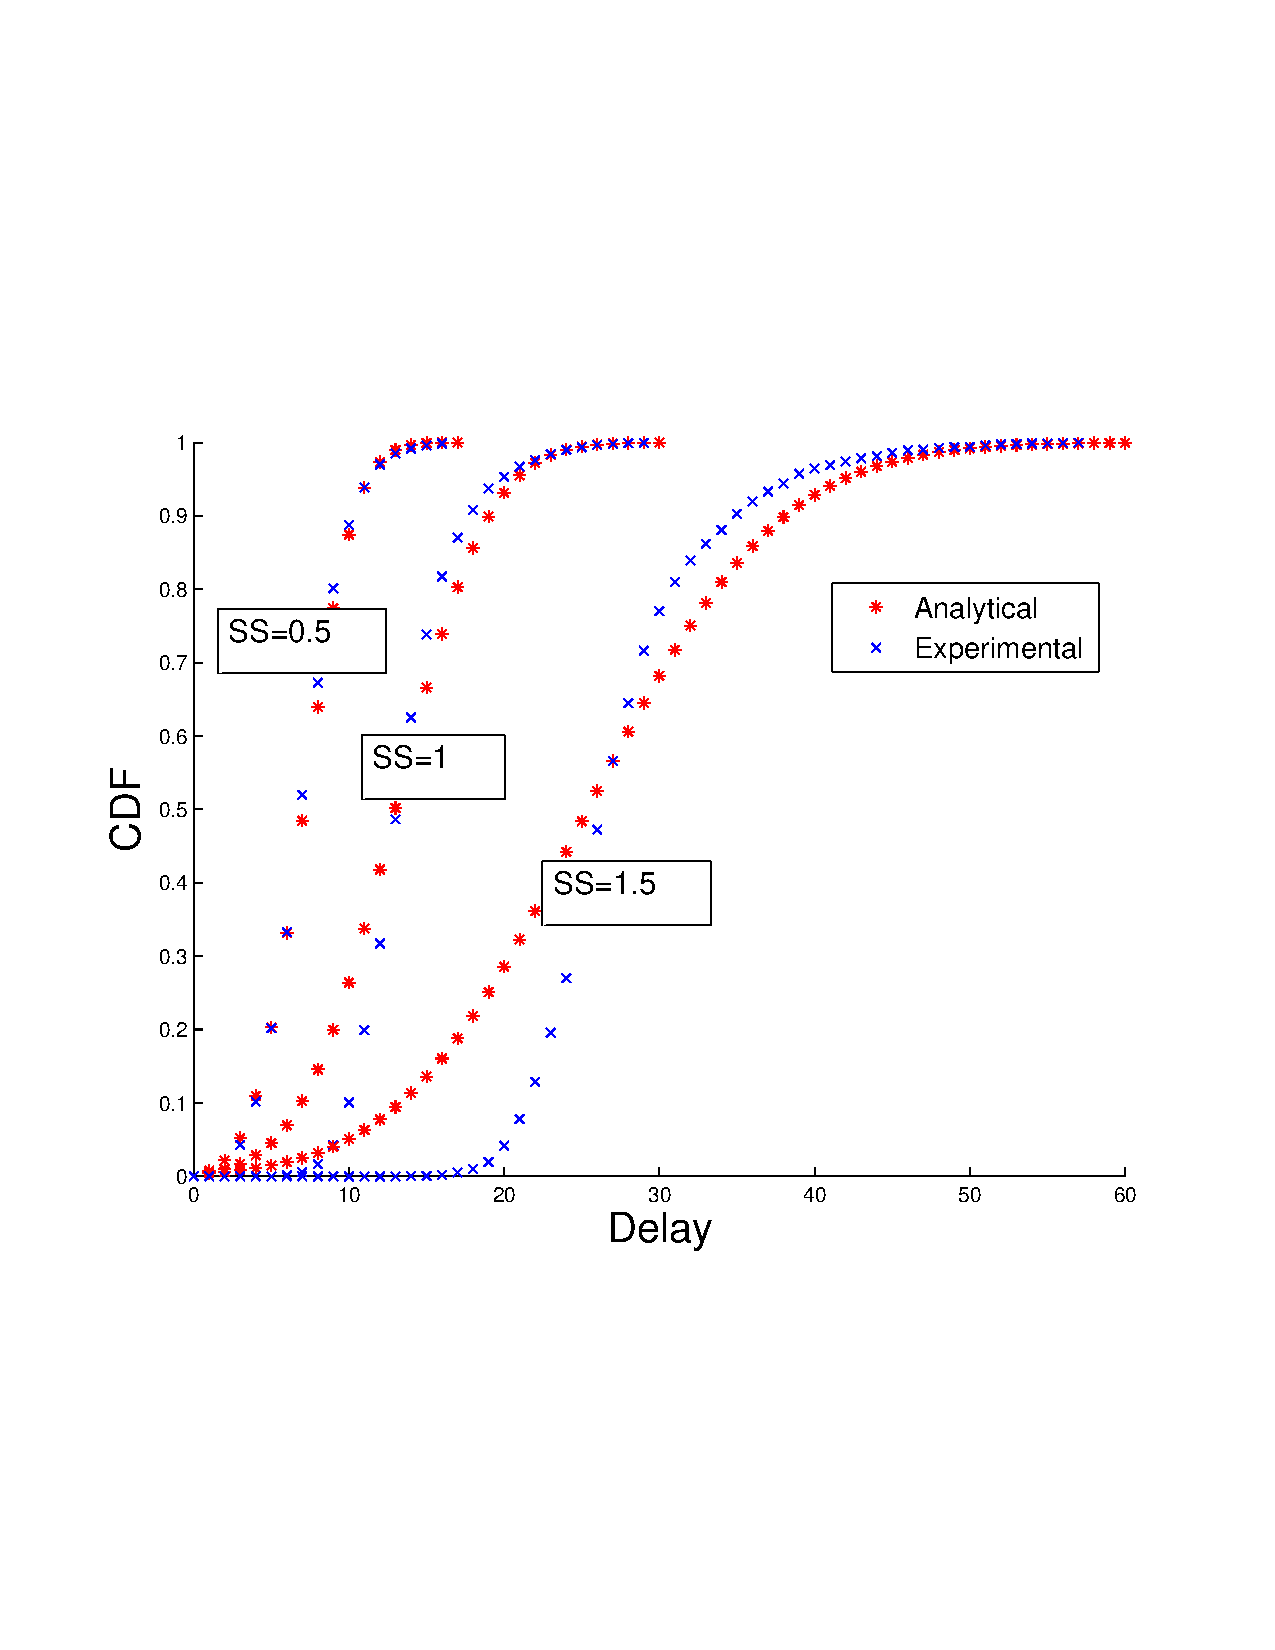
\includegraphics[scale=0.40, clip=true, trim=12mm 65mm 20mm 65mm]{figures/delay_cdfs/delay_cdf_grid.pdf}
        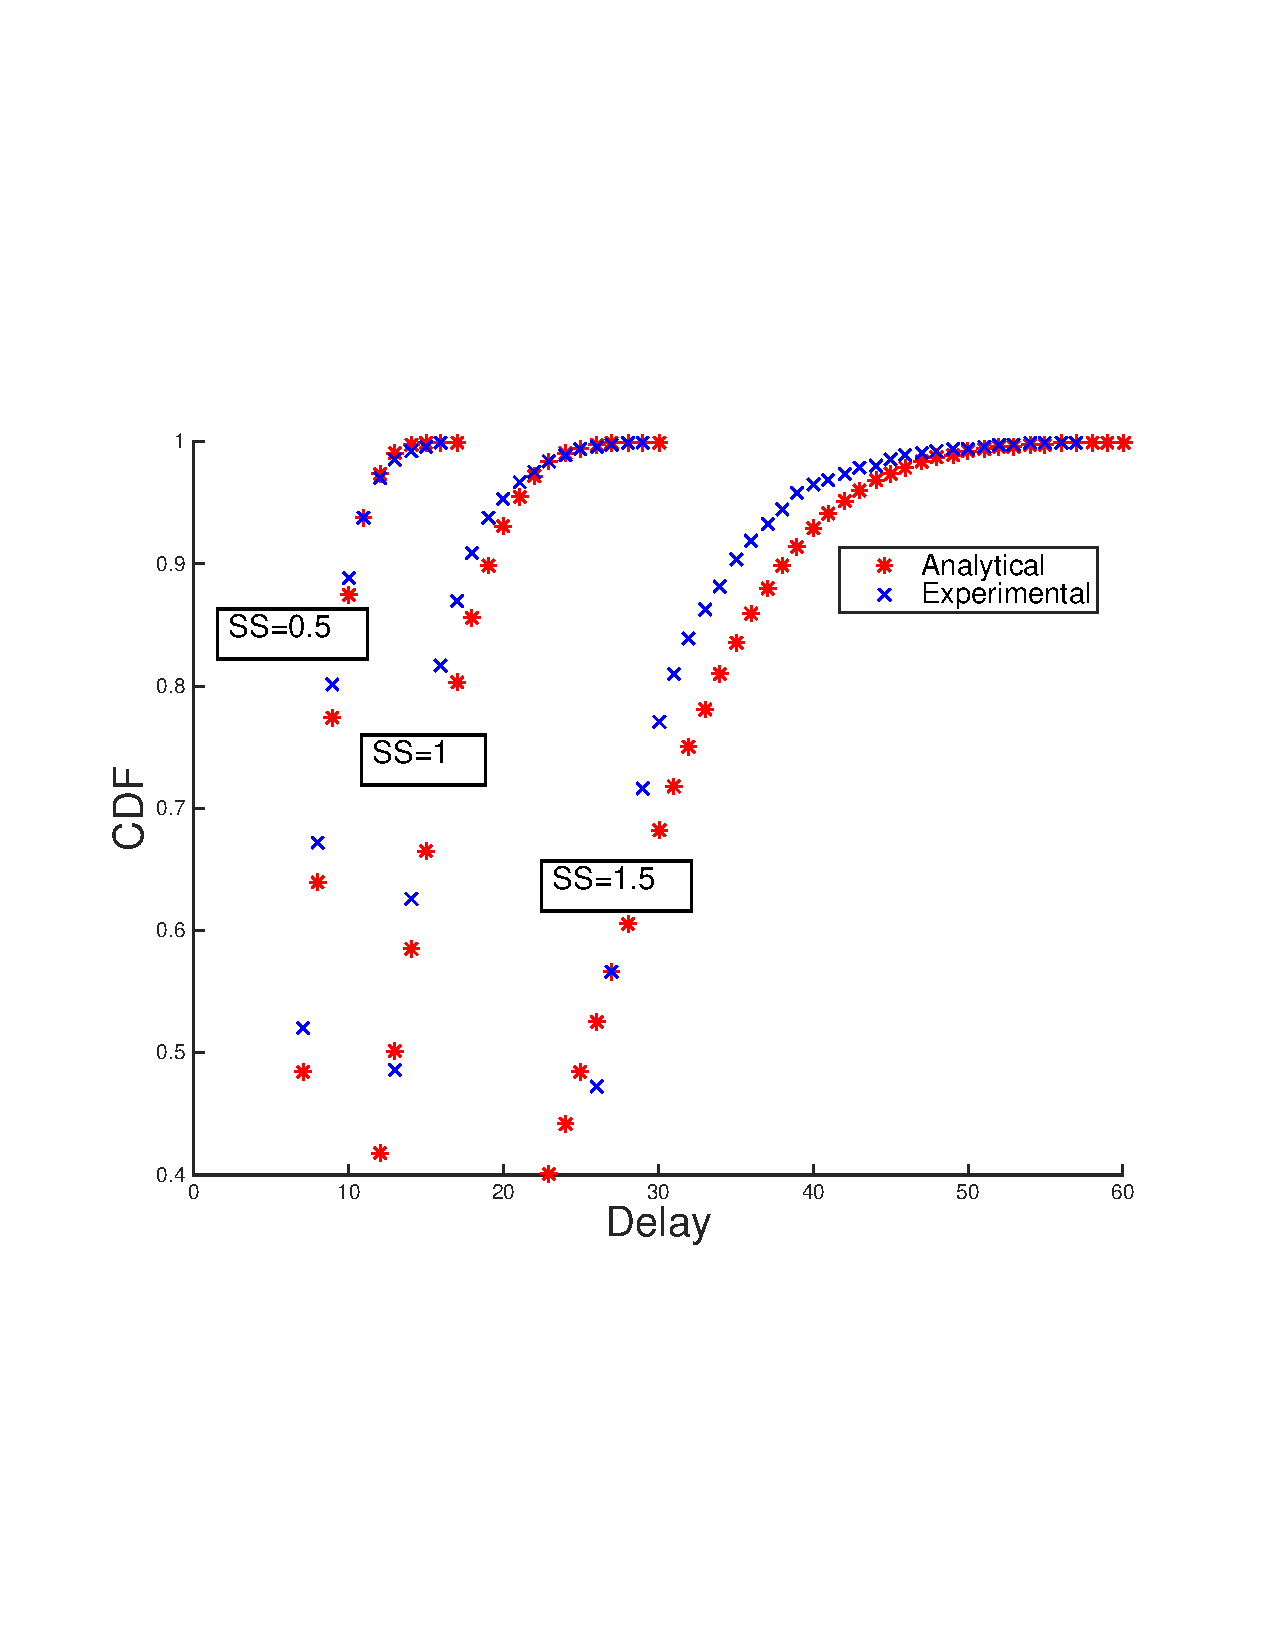
\includegraphics[scale=0.40, clip=true, trim=12mm 65mm 20mm 65mm]{figures/delay_cdfs/delay_cdf_grid_half.pdf}
        \label{fig:delay_cdf_grid}
        }
   \caption{Characterization of delay using framework follows distribution of empirical results in most cases.}
   \label{fig:delay_cdf_anal_vs_sim}
   \vspace{-4mm}
\end{figure}

\subsection{Probability of Timeliness Satisfiability}

While the minimum timeliness at which all flows are expected to complete before their deadlines can be determined by the scalability equations in Section \ref{sec:example_applications}, some applications may benefit from an understanding of what the probability of completing within the timeliness constraints for those below the minimum fully satisfiable timeliness.  For example, if a mission issues a number of queries for information to support decision-making, receiving $80\%$ or $90\%$ of the responses may be sufficient for making the decision.  The question of importance, then, is "How far can we reduce the timeliness constraint and still expect to receive $x\%$ of the queries in time?"  Or, equivalently, we may pose the question, "When the network is operating at the edge of capacity, what is the expected delay for $x\%$ of queries to be completed?"  Since equation \ref{eq:full_delay_cdf} provides the distribution of delays, it provides quality estimates to answer these questions.  

\subsection{Validation of Delay Characterization}

Figure \ref{fig:delay_cdf_anal_vs_sim} shows expected delay distributions from \ref{eq:full_delay_cdf} alongside distributions of delays recorded in ns3 simulations of the same networks.  We argue that minimum QoI requirements for most applications tend to be over $50\%$, and therefore focus on the top half of the delay distribution.  In all cases here, analytical predictions of satisfying the timeliness requirement are within about $10\%$ of empirical results for probabilities above $0.5$.  

These delay distributions also provide much more information about the expected delays of all queries in addition to the minimum satisfiable timeliness.  For each completeness requirement of a minimum expected Sum Similarity, the maximum delay at the top of the distribution provides the minimum satisfiable timeliness.  Examining the distributions, though, we see that many of the queries finish well before that maximum delay.  For example, focusing on the delay distribution when the Sum Similarity requirement is $1.5$ in Figure \ref{fig:delay_cdf_line}, we note that the maximum delay is approximately $45$ seconds, but $80\%$ of the queries on average finish in almost half of that delay.  
%Additionally, in smaller data load requirement cases, analytical predictions match simulation results quite closely along the entire distribution.

%\subsection{Scalability and Maximum QoI Equations}
%
%Once 

% from a different script:
%\subsubsection{Delay}
%
%The delay distribution for a flow beginning in source node $i$ is:
%
%\begin{equation}
%	f_{D_i} = \sum\limits_{j \neq i} [C_1 \cdot f_{TF_{i | j}}(tf) + C_2 \cdot PL(i,j)] \cdot p(j)
%\end{equation}
%which is equivalent to:
%\begin{equation}
%	P(D_i < d) = \sum\limits_{j \neq i} f_{TF_{i | j}}( \frac{d - C_2 \cdot PL(i,j)}{C_1} ) \cdot p(j)
%\end{equation}

%which can be expanded to:
%
%\begin{figure*}[t]
%\begin{eqnarray}
%\nonumber
%	f_{D_i} (d) = &&\frac{i}{N} \cdot \mathcal{N}( \frac{2(i-1)(N-i)}{(N-2)(N-1)} , \sqrt{\frac{2(i-1)(N-i)  (1-\frac{1}{N-1})}{(N-2)(N-1)}} )  \\ \nonumber
%			   &+& \sum\limits_{k=i}^{\frac{N}{2}-1} \cdot \frac{\frac{1}{2}-\frac{i}{N}}{\frac{N}{2} - i}\mathcal{N}( \frac{2(k-1)(N-k)}{(N-2)(N-1)}, \sqrt{\frac{2(k-1)(N-k)}{(N-2)(N-1)} (1-\frac{1}{N-1})} )  \\
%			   &+& \frac{1}{2} \cdot \mathcal{N} ( \frac{N(\frac{N}{2}-1)}{(N-2)(N-1)} , \sqrt{\frac{N(\frac{N}{2}-1)}{(N-2)(N-1)} (1-\frac{1}{N-1})} )
%\label{eq:full_PDF_TF_line_2}
%\end{eqnarray}
%\end{figure*}
% end from different script
